% chktex-file 9 chktex-file 17 chktex-file 36 chktex-file 3

\section{Exercise 2}
Consider the following 10 vertex graph and a random walk over these states

\begin{center}
    \def\edgebending{0cm}
\def\loopsize{0.5cm}
\definecolor{edgecolor}{RGB}{57, 0, 19}
\tikzstyle{matrix of math nodes}=[%
    matrix of nodes,
    nodes={%
     execute at begin node=$,%
     execute at end node=$%
    }%
  ]
\begin{tikzpicture}[scale=1.5,
    vertex/.style={fill = purple, circle, text = white, font=\bfseries},
    arc/.style={draw,ultra thick,->, shorten >=0.05cm, bend right = \edgebending, edgecolor},
    loop/.style={->, shorten > = 0.1cm, ultra thick, edgecolor}
    ]

    \newcommand{\coords}{
        (1.6030834721907683e-16, 2.618033988749895),
        (-0.587785252292473, 0.8090169943749475),
        (-2.48989828488278, 0.8090169943749477),
        (-0.9510565162951536, -0.3090169943749473),
        (-1.538841768587627, -2.1180339887498945),
        (-1.8369701987210297e-16, -1.0),
        (1.5388417685876261, -2.1180339887498953),
        (0.9510565162951535, -0.3090169943749476),
        (2.4898982848827806, 0.8090169943749468),
        (0.5877852522924734, 0.8090169943749472)
    }
    \newcommand{\adjmatrix}{
        {0, 1, 0, 0, 0, 0, 0, 0, 0, 1},
        {1, 0, 1, 1, 0, 0, 0, 0, 0, 1},
        {0, 1, 0, 1, 0, 0, 0, 0, 0, 0},
        {0, 1, 1, 0, 1, 1, 0, 0, 0, 0},
        {0, 0, 0, 1, 0, 1, 0, 0, 0, 0},
        {0, 0, 0, 1, 1, 0, 1, 1, 0, 0},
        {0, 0, 0, 0, 0, 1, 0, 1, 0, 0},
        {0, 0, 0, 0, 0, 1, 1, 0, 1, 1},
        {0, 0, 0, 0, 0, 0, 0, 1, 0, 1},
        {1, 1, 0, 0, 0, 0, 0, 1, 1, 0},
    }

    \newcommand{\labelmatrix}{
        {0, 1, 0, 0, 0, 0, 0, 0, 0, 1},
        {1, 0, 1, 1, 0, 0, 0, 0, 0, 1},
        {0, 1, 0, 1, 0, 0, 0, 0, 0, 0},
        {0, 1, 1, 0, 1, 1, 0, 0, 0, 0},
        {0, 0, 0, 1, 0, 1, 0, 0, 0, 0},
        {0, 0, 0, 1, 1, 0, 1, 1, 0, 0},
        {0, 0, 0, 0, 0, 1, 0, 1, 0, 0},
        {0, 0, 0, 0, 0, 1, 1, 0, 1, 1},
        {0, 0, 0, 0, 0, 0, 0, 1, 0, 1},
        {1, 1, 0, 0, 0, 0, 0, 1, 1, 0},
    }

    \newcommand{\getmatrixitem}[2]{%
    \StrBetween[#2,#1]{\labelmatrix}{, }{, }%
}


    % Define vertices
    \foreach [count = \i] \pos in \coords {
        \pgfmathsetmacro{\nodeangle}{round(90-atan2(\pos))}
        \ifnum\i=1
            \xdef\anglelist{\nodeangle}
        \else
            \xdef\anglelist{\anglelist,\nodeangle}
        \fi
        \coordinate[at=\pos, name=p\i];
        \pgfmathsetmacro{\nodename}{ }
        \node[vertex, at=\pos, name=V\i]{\nodename};
    }
        
    % Define edges
    \foreach [count = \i] \row in \labelmatrix{
    \foreach [count = \j] \edgelabel in \row{
        \pgfmathsetmacro{\weight}{{\adjmatrix}[\i-1][\j-1]}
        % Weight > 0
        \pgfmathsetmacro{\edgeexists}{\weight != 0 ? 1 : 0}
        \ifnum\edgeexists>0
            \pgfmathsetmacro{\isloop}{\i-\j == 0 ? 1 : 0}
            \ifnum\isloop>0
                \pgfmathsetmacro{\nodeangle}{{\anglelist}[\i-1]}
                \pgfmathsetmacro{\outangle}{int(\nodeangle - 50)}
                \pgfmathsetmacro{\inangle}{int(\nodeangle + 50)}
                \draw[loop] (V\i) to [in=\outangle,out=\inangle,looseness=\loopsize] node[] {} (V\i);
            \else
                \draw[arc] (V\i) to node[inner sep=1pt] {} (V\j);
            \fi            
        \fi
    }
    }
\end{tikzpicture}
\end{center}

\begin{enumerate}[label=(\alph*)]
    \item Enumerate the states $i$ by $\{0,\ldots, 9\}$ and assign to the time of the state exit, the rate $i+1$. Construct the $Q$-matrix of the resulting continuous time Markov chain.
    \item Calculate the invariant measure of this continuous time Markov chain.
    \item Build the transition matrix of the resulting discrete Markov chain.
    \item Calculate the invariant measure and compare with the measure of item (b).
    \item For item 2, simulate 100 trajectories of $[0,100]$ and approximate the invariant measure by the histograms of the visit period of each trajectory. Graph the trajectories, the histogram and the histogram of the visit times of each state.
    \item For item 4, simulate 100 trajectories of $[0,100]$ and approximate the invariant measure by the histograms of the visit period of each trajectory. Graph the trajectories, the histogram and the histogram of the visit times of each state.
\end{enumerate}

\subsection*{Solution Part (a)}

\textbf{Note:} For this solution, we are going to start counting from $i = 0$, and thus, the rate of the state $i$ is going to be $i+1$.

Beforehand, for the simulations and calculations, we are going to use Python with the following packages:

\begin{minted}{python3}
    import sympy as sp
    import numpy as np
    import scipy as sci
    import matplotlib.pyplot as plt
\end{minted}

\begin{center}
    \def\edgebending{0cm}
\def\loopsize{0.5cm}
\definecolor{edgecolor}{RGB}{57, 0, 19}
\tikzstyle{matrix of math nodes}=[%
    matrix of nodes,
    nodes={%
     execute at begin node=$,%
     execute at end node=$%
    }%
  ]
\begin{tikzpicture}[scale=0.7,
    vertex/.style={fill = purple, circle, text = white, font=\bfseries},
    arc/.style={draw,ultra thick,->, shorten >=0.05cm, bend right = \edgebending, edgecolor},
    loop/.style={->, shorten > = 0.1cm, ultra thick, edgecolor}
    ]

    \newcommand{\coords}{
        (7, -3),
        (-7, -3),
        (0, 5),
        (0, 2),
        (-3, -2),
        (3, -2)
    }

    \newcommand{\adjmatrix}{
        {0.0, 1.0, 0.0, 1.0, 0.0, 0.0},
        {0.0, 0.0, 1.0, 0.0, 0.0, 0.0},
        {1.0, 0.0, 0.0, 0.0, 0.0, 0.0},
        {0.0, 1.0, 1.0, 0.0, 1.0, 0.0},
        {0.0, 0.0, 0.0, 0.0, 0.0, 1.0},
        {0.0, 0.0, 0.0, 1.0, 0.0, 0.0},
    }

    \newcommand{\labelmatrix}{
        {0.0, 1/2, 0.0, 1/2, 0.0, 0.0},
        {0.0, 0.0, 1  , 0.0, 0.0, 0.0},
        {1  , 0.0, 0.0, 0.0, 0.0, 0.0},
        {0.0, 1/3, 1/3, 0.0, 1/3, 0.0},
        {0.0, 0.0, 0.0, 0.0, 0.0, 1  },
        {0.0, 0.0, 0.0, 1  , 0.0, 0.0},
    }

    \newcommand{\getmatrixitem}[2]{%
    \StrBetween[#2,#1]{\labelmatrix}{, }{, }%
}


    % Define vertices
    \foreach [count = \i] \pos in \coords {
        \pgfmathsetmacro{\nodeangle}{round(90-atan2(\pos))}
        \ifnum\i=1
            \xdef\anglelist{\nodeangle}
        \else
            \xdef\anglelist{\anglelist,\nodeangle}
        \fi
        \coordinate[at=\pos, name=p\i];
        \pgfmathsetmacro{\nodename}{int(\i-1)}
        \node[vertex, at=\pos, name=V\i]{\nodename};
    }
        
    % Define edges
    \foreach [count = \i] \row in \labelmatrix{
    \foreach [count = \j] \edgelabel in \row{
        \pgfmathsetmacro{\weight}{{\adjmatrix}[\i-1][\j-1]}
        % Weight > 0
        \pgfmathsetmacro{\edgeexists}{\weight != 0 ? 1 : 0}
        \ifnum\edgeexists>0
            \pgfmathsetmacro{\isloop}{\i-\j == 0 ? 1 : 0}
            \ifnum\isloop>0
                \pgfmathsetmacro{\nodeangle}{{\anglelist}[\i-1]}
                \pgfmathsetmacro{\outangle}{int(\nodeangle - 50)}
                \pgfmathsetmacro{\inangle}{int(\nodeangle + 50)}
                \draw[loop] (V\i) to [in=\outangle,out=\inangle,looseness=\loopsize] node[fill=white] {$\edgelabel$} (V\i);
            \else
                \draw[arc] (V\i) to node[fill=white, inner sep=1pt] {$\edgelabel$} (V\j);
            \fi            
        \fi
    }
    }
\end{tikzpicture}
\end{center}

The way we assign these numbers is arbitrary. The only important rules for the adjacency of this graph are, for $i \in \Z_5$:
\[ E_i \longleftrightarrow I_i,\hspace*{1em} E_i \longleftrightarrow I_{i-1},\hspace*{1em} I_i\longleftrightarrow I_{i-1}.   \]

However, for this exercise, we are going to enumerate the graph as follows:

\begin{center}
    \def\edgebending{0cm}
\def\loopsize{0.5cm}
\definecolor{edgecolor}{RGB}{57, 0, 19}
\tikzstyle{matrix of math nodes}=[%
    matrix of nodes,
    nodes={%
     execute at begin node=$,%
     execute at end node=$%
    }%
  ]
\begin{tikzpicture}[scale=1.5,
    vertex/.style={fill = purple, circle, text = white, font=\bfseries},
    arc/.style={draw,ultra thick,->, shorten >=0.05cm, bend right = \edgebending, edgecolor},
    loop/.style={->, shorten > = 0.1cm, ultra thick, edgecolor}
    ]

    \newcommand{\coords}{
        (1.6030834721907683e-16, 2.618033988749895),
        (-0.587785252292473, 0.8090169943749475),
        (-2.48989828488278, 0.8090169943749477),
        (-0.9510565162951536, -0.3090169943749473),
        (-1.538841768587627, -2.1180339887498945),
        (-1.8369701987210297e-16, -1.0),
        (1.5388417685876261, -2.1180339887498953),
        (0.9510565162951535, -0.3090169943749476),
        (2.4898982848827806, 0.8090169943749468),
        (0.5877852522924734, 0.8090169943749472)
    }
    \newcommand{\adjmatrix}{
        {0, 1, 0, 0, 0, 0, 0, 0, 0, 1},
        {1, 0, 1, 1, 0, 0, 0, 0, 0, 1},
        {0, 1, 0, 1, 0, 0, 0, 0, 0, 0},
        {0, 1, 1, 0, 1, 1, 0, 0, 0, 0},
        {0, 0, 0, 1, 0, 1, 0, 0, 0, 0},
        {0, 0, 0, 1, 1, 0, 1, 1, 0, 0},
        {0, 0, 0, 0, 0, 1, 0, 1, 0, 0},
        {0, 0, 0, 0, 0, 1, 1, 0, 1, 1},
        {0, 0, 0, 0, 0, 0, 0, 1, 0, 1},
        {1, 1, 0, 0, 0, 0, 0, 1, 1, 0},
    }

    \newcommand{\labelmatrix}{
        {0, 1, 0, 0, 0, 0, 0, 0, 0, 1},
        {1, 0, 1, 1, 0, 0, 0, 0, 0, 1},
        {0, 1, 0, 1, 0, 0, 0, 0, 0, 0},
        {0, 1, 1, 0, 1, 1, 0, 0, 0, 0},
        {0, 0, 0, 1, 0, 1, 0, 0, 0, 0},
        {0, 0, 0, 1, 1, 0, 1, 1, 0, 0},
        {0, 0, 0, 0, 0, 1, 0, 1, 0, 0},
        {0, 0, 0, 0, 0, 1, 1, 0, 1, 1},
        {0, 0, 0, 0, 0, 0, 0, 1, 0, 1},
        {1, 1, 0, 0, 0, 0, 0, 1, 1, 0},
    }

    \newcommand{\getmatrixitem}[2]{%
    \StrBetween[#2,#1]{\labelmatrix}{, }{, }%
}


    % Define vertices
    \foreach [count = \i] \pos in \coords {
        \pgfmathsetmacro{\nodeangle}{round(90-atan2(\pos))}
        \ifnum\i=1
            \xdef\anglelist{\nodeangle}
        \else
            \xdef\anglelist{\anglelist,\nodeangle}
        \fi
        \coordinate[at=\pos, name=p\i];
        \pgfmathsetmacro{\nodename}{int(\i-1)}
        \node[vertex, at=\pos, name=V\i]{\nodename};
    }
        
    % Define edges
    \foreach [count = \i] \row in \labelmatrix{
    \foreach [count = \j] \edgelabel in \row{
        \pgfmathsetmacro{\weight}{{\adjmatrix}[\i-1][\j-1]}
        % Weight > 0
        \pgfmathsetmacro{\edgeexists}{\weight != 0 ? 1 : 0}
        \ifnum\edgeexists>0
            \pgfmathsetmacro{\isloop}{\i-\j == 0 ? 1 : 0}
            \ifnum\isloop>0
                \pgfmathsetmacro{\nodeangle}{{\anglelist}[\i-1]}
                \pgfmathsetmacro{\outangle}{int(\nodeangle - 50)}
                \pgfmathsetmacro{\inangle}{int(\nodeangle + 50)}
                \draw[loop] (V\i) to [in=\outangle,out=\inangle,looseness=\loopsize] node[] {} (V\i);
            \else
                \draw[arc] (V\i) to node[inner sep=1pt] {} (V\j);
            \fi            
        \fi
    }
    }
\end{tikzpicture}
\end{center}

\begin{minted}{python3}
    exterior = [0,2,4,6,8]
    interior = [1,3,5,7,9]
    states = np.arange(10)
    adjacency = np.zeros((10,10))
    for i in range(5):
        adjacency[interior[i],exterior[i]] += 1
        adjacency[interior[i],exterior[(i-1)%5]] += 1
        adjacency[interior[i],interior[(i-1)%5]] += 1
    adjacency += adjacency.T
\end{minted}
\[ \hbox{Adj} = \left[\begin{matrix}0 & 1 & 0 & 0 & 0 & 0 & 0 & 0 & 0 & 1\\1 & 0 & 1 & 1 & 0 & 0 & 0 & 0 & 0 & 1\\0 & 1 & 0 & 1 & 0 & 0 & 0 & 0 & 0 & 0\\0 & 1 & 1 & 0 & 1 & 1 & 0 & 0 & 0 & 0\\0 & 0 & 0 & 1 & 0 & 1 & 0 & 0 & 0 & 0\\0 & 0 & 0 & 1 & 1 & 0 & 1 & 1 & 0 & 0\\0 & 0 & 0 & 0 & 0 & 1 & 0 & 1 & 0 & 0\\0 & 0 & 0 & 0 & 0 & 1 & 1 & 0 & 1 & 1\\0 & 0 & 0 & 0 & 0 & 0 & 0 & 1 & 0 & 1\\1 & 1 & 0 & 0 & 0 & 0 & 0 & 1 & 1 & 0\end{matrix}\right] \]

Since there is no loop in the graph, the jump matrix (Denoted by $\Pi$) of this process can be is obtained from the adjacency matrix with each row being divided by the row sum:
\begin{minted}{python3}
    jump_matrix = adjacency / adjacency.sum(axis=1)[:,None]
\end{minted}
\[ \Pi = \left[\begin{matrix}0 & \frac{1}{2} & 0 & 0 & 0 & 0 & 0 & 0 & 0 & \frac{1}{2}\\\frac{1}{4} & 0 & \frac{1}{4} & \frac{1}{4} & 0 & 0 & 0 & 0 & 0 & \frac{1}{4}\\0 & \frac{1}{2} & 0 & \frac{1}{2} & 0 & 0 & 0 & 0 & 0 & 0\\0 & \frac{1}{4} & \frac{1}{4} & 0 & \frac{1}{4} & \frac{1}{4} & 0 & 0 & 0 & 0\\0 & 0 & 0 & \frac{1}{2} & 0 & \frac{1}{2} & 0 & 0 & 0 & 0\\0 & 0 & 0 & \frac{1}{4} & \frac{1}{4} & 0 & \frac{1}{4} & \frac{1}{4} & 0 & 0\\0 & 0 & 0 & 0 & 0 & \frac{1}{2} & 0 & \frac{1}{2} & 0 & 0\\0 & 0 & 0 & 0 & 0 & \frac{1}{4} & \frac{1}{4} & 0 & \frac{1}{4} & \frac{1}{4}\\0 & 0 & 0 & 0 & 0 & 0 & 0 & \frac{1}{2} & 0 & \frac{1}{2}\\\frac{1}{4} & \frac{1}{4} & 0 & 0 & 0 & 0 & 0 & \frac{1}{4} & \frac{1}{4} & 0\end{matrix}\right]
\]

For the generator matrix of this process (denoted by $Q$), note that the holding rates, according to the exercise, are $q_i = i+1$ for the state $i$. Thus, the diagonal of this matrix should be $-q_i = -(i+1)$. The other entries in each row have equal weight, so $q_{i,j} = \pi_{i,j}/q_i$:
\begin{minted}{python3}
    holding_rates = np.array([i+1 for i in range(10)])
    Q_matrix = -np.diag(holding_rates).astype(float)
    Q_matrix += adjacency * (holding_rates / adjacency.sum(axis=1))[:,None]
\end{minted}
\[ Q = \left[\begin{matrix}-1 & \frac{1}{2} & 0 & 0 & 0 & 0 & 0 & 0 & 0 & \frac{1}{2}\\\frac{1}{2} & -2 & \frac{1}{2} & \frac{1}{2} & 0 & 0 & 0 & 0 & 0 & \frac{1}{2}\\0 & \frac{3}{2} & -3 & \frac{3}{2} & 0 & 0 & 0 & 0 & 0 & 0\\0 & 1 & 1 & -4 & 1 & 1 & 0 & 0 & 0 & 0\\0 & 0 & 0 & \frac{5}{2} & -5 & \frac{5}{2} & 0 & 0 & 0 & 0\\0 & 0 & 0 & \frac{3}{2} & \frac{3}{2} & -6 & \frac{3}{2} & \frac{3}{2} & 0 & 0\\0 & 0 & 0 & 0 & 0 & \frac{7}{2} & -7 & \frac{7}{2} & 0 & 0\\0 & 0 & 0 & 0 & 0 & 2 & 2 & -8 & 2 & 2\\0 & 0 & 0 & 0 & 0 & 0 & 0 & \frac{9}{2} & -9 & \frac{9}{2}\\\frac{5}{2} & \frac{5}{2} & 0 & 0 & 0 & 0 & 0 & \frac{5}{2} & \frac{5}{2} & -10\end{matrix}\right]
\]

\subsection*{Solution Part (b)}

In order to find the left eigenvector associated with an specific eigenvalue, we designed the following function:

\begin{minted}{python3}
    def get_left_eigenvector(matrix, desired_eigenvalue):
        eigenvalues, multiplicity, eigenvectors = list(zip(*sp.Matrix(matrix.T).eigenvects()))

        solution_index = np.argmin(np.abs(desired_eigenvalue - np.array(eigenvalues)))
        solution = eigenvectors[solution_index][0]
        solution = solution / sum(solution)
        return sp.nsimplify(solution.T.simplify(), tolerance=0.0001, rational= True)
\end{minted}

The invariant distribution $\lambda$ associated to this continuous process can be obtained using many methods. In fact, it's the solution to the following equations:
\[ \everymath{\displaystyle}
\arraycolsep=4pt\def\arraystretch{2.5}
\begin{array}{rcl}
    (1): & \mu\Pi = \mu, & \lambda_i = \frac{\mu_i/q_i}{\sum_{i = 1}^{|I|} \mu_i/q_i}\\
    (2): & \lambda Q = 0\\
    (3): & \lambda P(t) = \lambda, & P(t) = e^{tQ},\; \forall t\geq 0
\end{array}\]

\subsubsection*{Method (1)}
For method (1), we obtain
\begin{minted}{python3}
    mu_invariant = get_left_eigenvector(jump_matrix, 1)
\end{minted}
\[ \mu = \left[\begin{matrix}\frac{1}{15} & \frac{2}{15} & \frac{1}{15} & \frac{2}{15} & \frac{1}{15} & \frac{2}{15} & \frac{1}{15} & \frac{2}{15} & \frac{1}{15} & \frac{2}{15}\end{matrix}\right]
\]
\begin{minted}{python3}
    lambda_invariant_1 = mu_invariant/holding_rates
    lambda_invariant_1 = lambda_invariant_1/lambda_invariant_1.sum()
\end{minted}
\[ \lambda_1 = \left[\begin{matrix}\frac{1260}{5129} & \frac{1260}{5129} & \frac{420}{5129} & \frac{630}{5129} & \frac{252}{5129} & \frac{420}{5129} & \frac{180}{5129} & \frac{315}{5129} & \frac{140}{5129} & \frac{252}{5129}\end{matrix}\right].
\]

\subsubsection*{Method (2)}
Then, for the next method, we have
\begin{minted}{python3}
    lambda_invariant_2 = get_left_eigenvector(Q_matrix, 0)
\end{minted}
\[ \lambda_2 = \left[\begin{matrix}\frac{1260}{5129} & \frac{1260}{5129} & \frac{420}{5129} & \frac{630}{5129} & \frac{252}{5129} & \frac{420}{5129} & \frac{180}{5129} & \frac{315}{5129} & \frac{140}{5129} & \frac{252}{5129}\end{matrix}\right]. \]

\subsubsection*{Method (3)}
Finally, for the last method, we set $t = 1$ to calculate $P(1) = e^Q$
\begin{minted}{python3}
    P_matrix = sci.linalg.expm(Q_matrix)
    lambda_invariant_3 = get_left_eigenvector(P_matrix, 1)
\end{minted}
Yet again, we obtain the same results:
\[ \lambda_3 = \left[\begin{matrix}\frac{1260}{5129} & \frac{1260}{5129} & \frac{420}{5129} & \frac{630}{5129} & \frac{252}{5129} & \frac{420}{5129} & \frac{180}{5129} & \frac{315}{5129} & \frac{140}{5129} & \frac{252}{5129}\end{matrix}\right]. \]

Therefore, we can be sure that the invariant distribution of this process is 
\[\begin{array}{rcl}
    \lambda & = & \left[\begin{matrix}\frac{1260}{5129} & \frac{1260}{5129} & \frac{420}{5129} & \frac{630}{5129} & \frac{252}{5129} & \frac{420}{5129} & \frac{180}{5129} & \frac{315}{5129} & \frac{140}{5129} & \frac{252}{5129}\end{matrix}\right]\\[5mm]
    & \approx &  \mathtt{\text{[0.246\; 0.246\; 0.082\; 0.123\; 0.049\; 0.082\; 0.035\; 0.061\; 0.027\; 0.049]}}.
\end{array} \]

\subsection*{Solution Part (c)}
The matrix the exercise is asking for has diagonal $\gamma_{ii} = 1-\frac{1}{q_i}$. That is because a success, which is to exit state i, has probability $\frac{1}{q_i}$. Therefore, to exit a given state, has distribution $\hbox{Geo}(\frac{1}{q_i})$. It follows that the other row entries (excluding the diagonal) should collectively sum $\frac{1}{q_i}$:
\[ \sum_{j \in I}\gamma_{ij} = \gamma_{ii} + \sum_{j \neq i} \gamma_{ij} = 1 \]
\[ \implies \sum_{j \neq i} \gamma_{ij} = \frac{1}{q_i}. \]
For these probabilities to be correctly weighted according to the graph, the closed formula for $\gamma_{ij}$ is
\[ \gamma_{ij} = \pi_{ij} \cdot \frac{1}{q_i}. \]
Therefore,
\begin{minted}{python3}
    transition_matrix = np.diag(1-1/holding_rates)
    transition_matrix += jump_matrix * (1/holding_rates)[:,None]
\end{minted}
\[ \Gamma = \left[\begin{matrix}0 & \frac{1}{2} & 0 & 0 & 0 & 0 & 0 & 0 & 0 & \frac{1}{2}\\\frac{1}{8} & \frac{1}{2} & \frac{1}{8} & \frac{1}{8} & 0 & 0 & 0 & 0 & 0 & \frac{1}{8}\\0 & \frac{1}{6} & \frac{2}{3} & \frac{1}{6} & 0 & 0 & 0 & 0 & 0 & 0\\0 & \frac{1}{16} & \frac{1}{16} & \frac{3}{4} & \frac{1}{16} & \frac{1}{16} & 0 & 0 & 0 & 0\\0 & 0 & 0 & \frac{1}{10} & \frac{4}{5} & \frac{1}{10} & 0 & 0 & 0 & 0\\0 & 0 & 0 & \frac{1}{24} & \frac{1}{24} & \frac{5}{6} & \frac{1}{24} & \frac{1}{24} & 0 & 0\\0 & 0 & 0 & 0 & 0 & \frac{1}{14} & \frac{6}{7} & \frac{1}{14} & 0 & 0\\0 & 0 & 0 & 0 & 0 & \frac{1}{32} & \frac{1}{32} & \frac{7}{8} & \frac{1}{32} & \frac{1}{32}\\0 & 0 & 0 & 0 & 0 & 0 & 0 & \frac{1}{18} & \frac{8}{9} & \frac{1}{18}\\\frac{1}{40} & \frac{1}{40} & 0 & 0 & 0 & 0 & 0 & \frac{1}{40} & \frac{1}{40} & \frac{9}{10}\end{matrix}\right]
\]

\subsection*{Solution Part (d)}

The invariant distribution $\nu$ for this process is the solution of the following system
\[ \nu \Gamma = \nu. \]
\begin{minted}{python3}
    transition_invariant = get_left_eigenvector(transition_matrix, 1)
\end{minted}
\[ \begin{array}{rcl}
    \nu & = & \left[\begin{matrix}\frac{1}{85} & \frac{4}{85} & \frac{3}{85} & \frac{8}{85} & \frac{1}{17} & \frac{12}{85} & \frac{7}{85} & \frac{16}{85} & \frac{9}{85} & \frac{4}{17}\end{matrix}\right].\\[5mm]
    & \approx & [0.012\; 0.047\; 0.035\; 0.094\; 0.059\; 0.141\; 0.082\; 0.188\; 0.106\; 0.235]
\end{array} \]

This measure seems to have no relation with the other process

\subsection*{Solution Part (e)}

We have a sequence $(X^j,T^j)_{j\in\N}$ of steps in one trajectory. Assume that $m$ is the total number of jumps that the process makes before stopping at the time $T$. Then, for such trajectory we can define $X_t$ as follows
\[ 0 = T^0 < \cdots < T^m \leq T, \]
\[ X_t = X^j,\hspace*{1em} \hbox{for } t \in [T^j, T^{j+1}) \]
\[ \P\{X^{j+1} = l \;|\; X^{j} = k, \ldots, X^0 = k_0\} = \P\{X^{j+1} = l \;|\; X^{j} = k\} = \pi_{kl}. \]
The last property is the Markov property. Finally, $T^k$ is independent from $X^l$ for every $k,l\in\N$, and $T^j \sim \hbox{Exp}(q_{X^j})$. We are going to simulate this process $N$ times:

\begin{minted}{python3}
    T = 100 # max time
    N = 100 # number of trajectories
    trajectories = []

    for trajectory_index in range(N): # simulating N trajectories
        current_time = 0
        time_list = [current_time]
        state_list = [np.random.choice(states, p=mu_invariant)]

        while current_time < T:
            current_state = state_list[-1]
            current_rate = holding_rates[current_state]
            current_time += np.random.exponential(scale=1/holding_rates[current_state])
            time_list.append(current_time)
            next_state = np.random.choice(states, p=jump_matrix[current_state])
            state_list.append(next_state)
        state_list = np.array(state_list)
        time_list = np.array(time_list)
        trajectories.append((time_list, state_list))
\end{minted}
\textbf{Note:} We started the simulation with $X_0 \sim \mu$. The results are the following,

\begin{figure}[H]
    \centering
    \begin{minipage}[b]{0.49\textwidth}
        \centering
        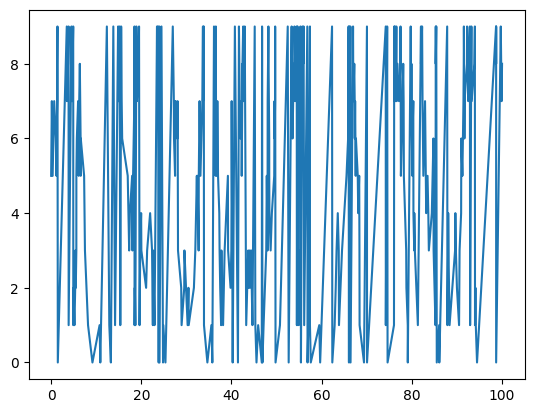
\includegraphics[width=\textwidth]{../pictures/2.e.9.png}
        \caption*{1 trajectory graph}
    \end{minipage}
    \hfill
    \begin{minipage}[b]{0.49\textwidth}
        \centering
        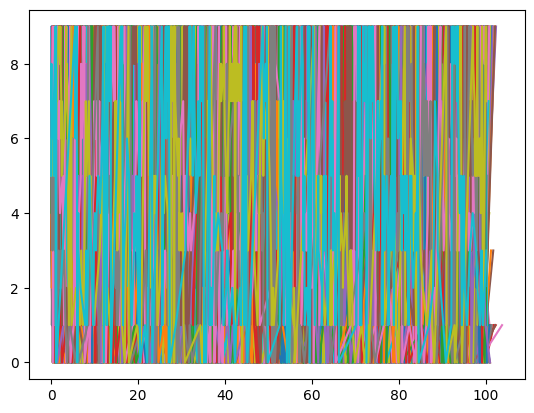
\includegraphics[width=\textwidth]{../pictures/2.e.10.png}
        \caption*{The graph mess for all the trajectories}
    \end{minipage}
\end{figure}


\subsubsection*{Estimating $\boldsymbol{\mu}$ with the frequencies}

Our estimator for $\mu$ is going to be
\[ \wh{\mu}_i = \frac{1}{m}\sum_{j = 0}^{m} \1(X^j = i). \]
This is the average number of times that our process jumps to the state $i$, and since the Markov process $X^j$ is independent from $T^j$, it follows from the ergodic theorem that $\wh{\mu}_i \to \mu$ as $m$ goes to infinity.
\begin{minted}{python3}
    def get_visit_frequency(trajectory):
        trajectory = trajectories[0]
        time_list, state_list = trajectory
        state_list = state_list[:-1]
        values, indices, counts = np.unique(state_list[state_list.argsort()], 
            return_counts=True, return_index=True)
        
        visit_frequency = counts/counts.sum()
        return visit_frequency
\end{minted}
To produce a comparison, we make an average of this visit frequency from the list of all the trajectories,
\begin{minted}{python3}
    visit_frequencies = np.array([get_visit_frequency(trajectory) 
        for trajectory in trajectories])
    average_visit_frequency = visit_frequencies.mean(axis = 0)

    bar_width = 0.35
    x = range(len(average_visit_frequency))

    fig, ax = plt.subplots()
    bar1 = ax.bar(x, average_visit_frequency, bar_width,
        label=r'$\wh{\mu}_i = \frac{1}{m}\sum_{j = 0}^{m} 1(X^j = i)$')
    bar2 = ax.bar([i + bar_width for i in x], mu_invariant, bar_width, label=r"$\mu_i$")

    ax.set_xticks([i + bar_width / 2 for i in x])
    ax.set_xticklabels([str(i) for i in range(len(average_visit_frequency))])
\end{minted}

\begin{figure}[H]
    \centering
    \begin{minipage}[b]{0.49\textwidth}
        \centering
        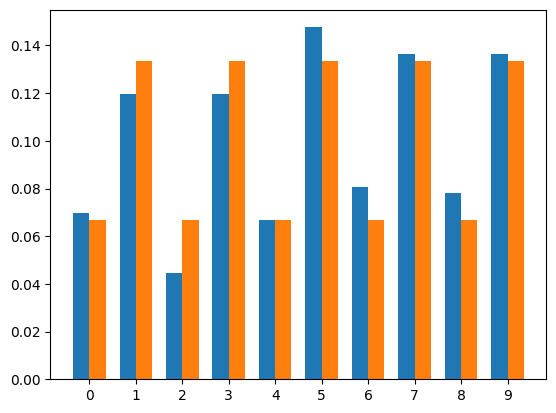
\includegraphics[width=\textwidth]{../pictures/2.e.1.png}
        \caption*{$N = 100,\; T = 100$}
    \end{minipage}
    \hfill
    \begin{minipage}[b]{0.49\textwidth}
        \centering
        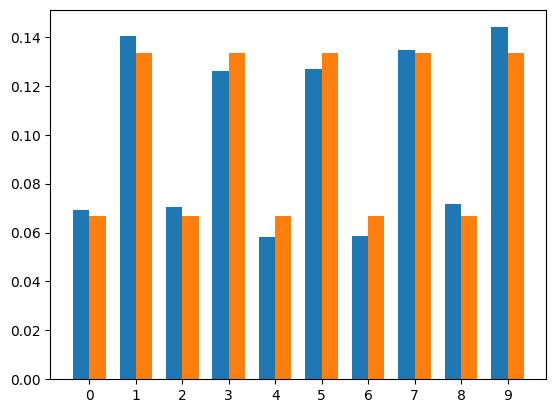
\includegraphics[width=\textwidth]{../pictures/2.e.2.png}
        \caption*{$N = 100,\; T = 1000$}
    \end{minipage}
    \caption*{The {\color{blue} blue bar (left)} is the result of the estimator {\color{blue}$\boldsymbol{\wh{\mu}_i}$} simulated $N=100$ times.\\ The {\color{red} orange bar (right)} is real value of the invariant measure {\color{red}$\boldsymbol{\mu_i}$}. }
\end{figure}

\subsubsection*{Estimating $\boldsymbol{q_i}$ with the visit lengths}

Let $T^n_i$ be the time of the $n$-th return to the state $i$. Also, let $M^n_i$ be the length of the $n$-th visit to $i$. In other words,
\[ M^n_i = \inf\{t > T^n_i : X_t \neq i\} - T^n_i. \]
According to the ergodic theorem,
\[\frac{M^1_i + \cdots + M^n_i}{n} \to \frac{1}{q_i},\; \hbox{as }n\to\infty. \]
Thus, we can propose an estimator
\[ \wh{q}_i = \left( \frac{M^1_i + \cdots + M^{n_i}_i}{n_i} \right)^{-1}, \]
where $n_i$ is the last time that we visit $i$ before $T$.

\begin{minted}{python3}
    def get_average_visit_length(trajectory):
        trajectory = trajectories[0]
        time_list, state_list = trajectory
        state_list = state_list[:-1]
        visit_lengths = time_list[1:] - time_list[:-1]
        values, indices, counts = np.unique(state_list[state_list.argsort()], 
            return_counts=True, return_index=True)
        visit_times_grouped = np.split(time_list[:-1][state_list.argsort()], indices)[1:] 
        visit_times_grouped = [np.sort(visit_times_grouped[k]) for k in range(10)]
        visit_lengths_grouped = np.split(visit_lengths[state_list.argsort()], indices)[1:] 

        average_visit_length = np.array([visit_lengths_grouped[k].mean() for k in range(10)])
        return average_visit_length
\end{minted}

After making an average of the $N = 100$ simulations of this estimator, we obtain

\begin{minted}{python3}
    average_visit_length = np.array([get_average_visit_length(trajectory) 
        for trajectory in trajectories]).mean(axis = 0)
    expected_visit_lengths = [1/holding_rates[k] for k in range(10)]
    bar_width = 0.35
    x = range(len(average_visit_length))

    fig, ax = plt.subplots()
    bar1 = ax.bar(x, average_visit_length, bar_width, 
        label=r'$\dfrac{1}{n}\sum_{k = 1}^n M_i^k$')
    bar2 = ax.bar([i + bar_width for i in x], expected_visit_lengths, bar_width,
        label=r"$\dfrac{1}{q_i}$")

    ax.set_xticks([i + bar_width / 2 for i in x])
    ax.set_xticklabels([str(i) for i in range(len(average_visit_length))])
    ax.legend()
\end{minted}

\begin{figure}[H]
    \centering
    \begin{minipage}[b]{0.49\textwidth}
        \centering
        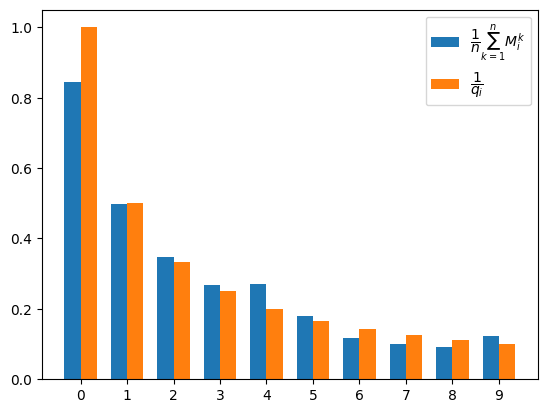
\includegraphics[width=\textwidth]{../pictures/2.e.3.png}
        \caption*{$N = 100,\; T = 100$}
    \end{minipage}
    \hfill
    \begin{minipage}[b]{0.49\textwidth}
        \centering
        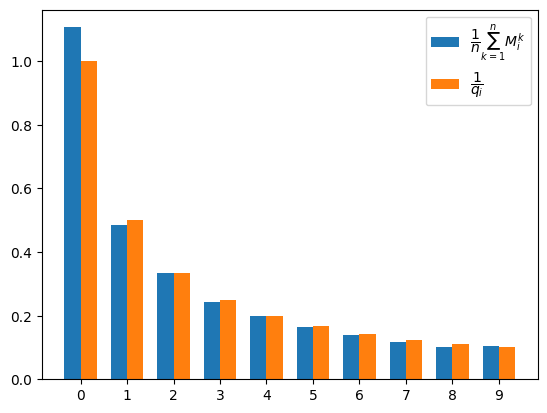
\includegraphics[width=\textwidth]{../pictures/2.e.4.png}
        \caption*{$N = 100,\; T = 1000$}
    \end{minipage}
    \caption*{The {\color{blue} blue bar (left)} is the result of the estimator {\color{blue}$\boldsymbol{\wh{q}_i}$} simulated $N = 100$ times.\\ The {\color{red} orange bar (right)} is real value of the holding rate {\color{red}$\boldsymbol{q_i}$}. }
\end{figure}

\subsubsection*{Estimating $\boldsymbol{\lambda_i}$ with $\boldsymbol{\wh{\mu}_i}$ and $\boldsymbol{\wh{q}_i}$}

\[\lambda_i = \frac{\mu_i/q_i}{\sum_{i = 1}^{|I|} \mu_i/q_i}. \]
Thus, with the previous results, we can make an estimator of $\lambda$ with
\[ \wh{\lambda}_i = \frac{\wh{\mu}_i/\wh{q}_i}{\sum_{i = 1}^{|I|} \wh{\mu}_i/\wh{q_i}} \]

\begin{minted}{python3}
    lambda_estimated_1 = average_visit_frequency*average_visit_length
    lambda_estimated_1 = lambda_estimated_1 / lambda_estimated_1.sum()

    bar_width = 0.35
    x = range(len(lambda_estimated_1))

    fig, ax = plt.subplots()
    bar1 = ax.bar(x, lambda_estimated_1, bar_width, label=r'$\hat{\lambda}_i$')
    bar2 = ax.bar([i + bar_width for i in x], lambda_invariant, bar_width, label=r"$\lambda_i$")

    ax.set_xticks([i + bar_width / 2 for i in x])
    ax.set_xticklabels([str(i) for i in range(len(lambda_estimated_1))])
    ax.legend()
\end{minted}

\begin{figure}[H]
    \centering
    \begin{minipage}[b]{0.49\textwidth}
        \centering
        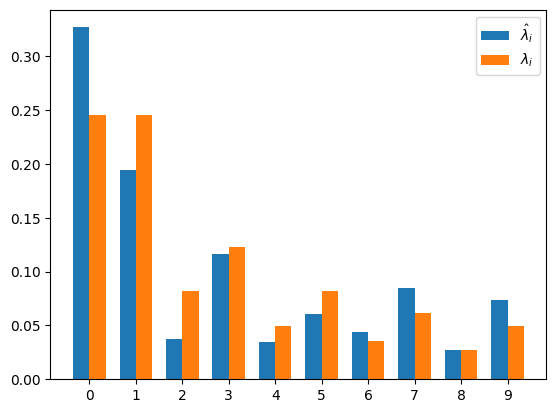
\includegraphics[width=\textwidth]{../pictures/2.e.6.png}
        \caption*{$N = 100,\; T = 100$}
    \end{minipage}
    \hfill
    \begin{minipage}[b]{0.49\textwidth}
        \centering
        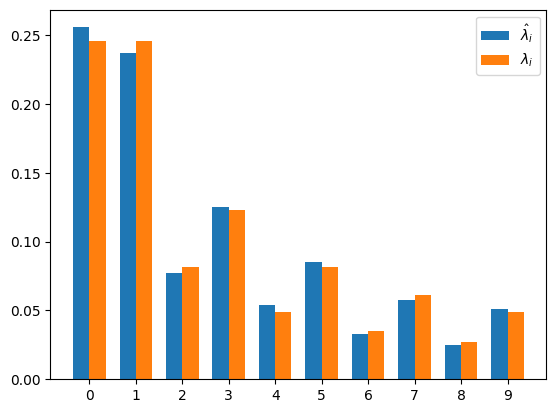
\includegraphics[width=\textwidth]{../pictures/2.e.5.png}
        \caption*{$N = 100,\; T = 1000$}
    \end{minipage}
    \caption*{The {\color{blue} blue bar (left)} is the result of the estimator {\color{blue}$\boldsymbol{\wh{\lambda}_i}$} simulated $N = 100$ times.\\ The {\color{red} orange bar (right)} is real value of the invariant measure {\color{red}$\boldsymbol{\lambda_i}$}. }
\end{figure}

\subsubsection*{My favorite way to estimate $\boldsymbol{\lambda}$}

We define the $n$-th excursion time $L_i^n$ to the state $i$ as the difference between return times:
\[ L^n_i = T_i^{n+1} - T_i^{n} \]
According to the ergodic theorem,
\[ \wh{m}_i = \frac{L^1_i + \cdots + L^n_i}{n} \to m_i = \E[T_i],\; \hbox{as }n\to\infty. \]
where $m_i$ is the expected return time to the state $i$. Since $\lambda_i = \frac{1}{m_i q_i}$, we can also produce another estimator

\[ \lambda^*_i = \frac{1}{\wh{m_i} \wh{q_i}} = \frac{M^1_i + \cdots + M^n_i}{L^1_i + \cdots + L^n_i} \]

First we define the function for the average excursion times:
\begin{minted}{python3}
    def get_average_excursion_length(trajectory):
        time_list, state_list = trajectory
        state_list = state_list[:-1]
        visit_lengths = time_list[1:] - time_list[:-1]
        values, indices, counts = np.unique(state_list[state_list.argsort()],
            return_counts=True, return_index=True)

        visit_times_grouped = np.split(time_list[:-1][state_list.argsort()], indices)[1:] 
        visit_times_grouped = [np.sort(visit_times_grouped[k])
        for k in range(10)]
        excursion_lengths_grouped = [
            visit_times_grouped[k][1:]- visit_times_grouped[k][:-1] for k in range(10)
            ]

        average_excursion_length = np.array(
            [excursion_lengths_grouped[k].mean() for k in range(10)])
        return average_excursion_length
\end{minted}

Now we create the estimator and compare it with the real $\lambda$

\begin{minted}{python3}
    average_excursion_length = np.array(
        [get_average_excursion_length(trajectory) for trajectory in trajectories]
        ).mean(axis = 0)

    lambda_estimated_2 = average_visit_length/average_excursion_length
    
    bar_width = 0.35
    x = range(len(lambda_estimated_2))
    
    fig, ax = plt.subplots()
    bar1 = ax.bar(x, lambda_estimated_2, bar_width, label=r'$\hat{\lambda}_i$')
    bar2 = ax.bar([i + bar_width for i in x],
        lambda_invariant, bar_width, label=r"$\lambda_i$")
    
    ax.set_xticks([i + bar_width / 2 for i in x])
    ax.set_xticklabels([str(i) for i in range(len(lambda_estimated_2))])
    ax.legend()
\end{minted}

\begin{figure}[H]
    \centering
    \begin{minipage}[b]{0.49\textwidth}
        \centering
        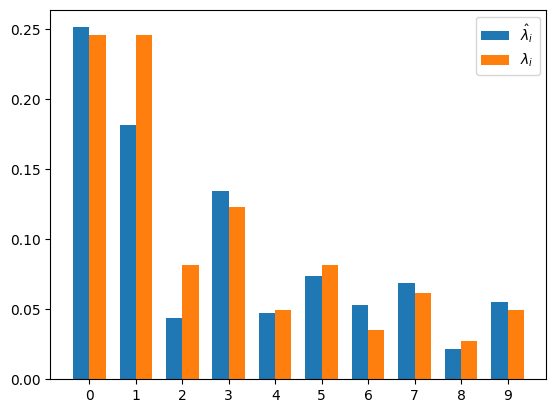
\includegraphics[width=\textwidth]{../pictures/2.e.8.png}
        \caption*{$N = 100,\; T = 100$}
    \end{minipage}
    \hfill
    \begin{minipage}[b]{0.49\textwidth}
        \centering
        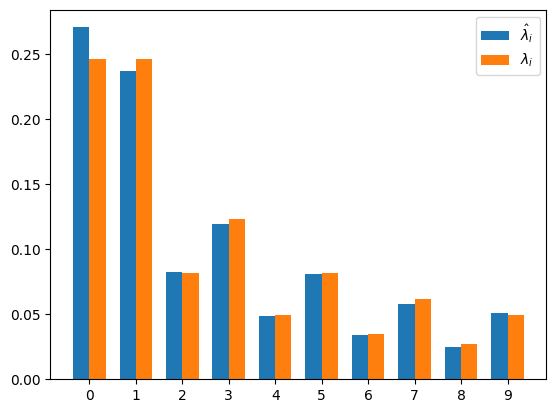
\includegraphics[width=\textwidth]{../pictures/2.e.7.png}
        \caption*{$N = 100,\; T = 1000$}
    \end{minipage}
    \caption*{The {\color{blue} blue bar (left)} is the result of the estimator {\color{blue}$\boldsymbol{\lambda_i^*}$} simulated $N = 100$ times.\\ The {\color{red} orange bar (right)} is real value of the invariant measure {\color{red}$\boldsymbol{\lambda_i}$}. }
\end{figure}

\subsection*{Solution Part (f)}

Now, for the discrete process related to the matrix $\Gamma$, we simulate $N = 100$ trajectories of $T = 100$ steps

\begin{minted}{python3}
    T = 100 # max time
    N = 100 # number of trajectories
    trajectories = []
    
    for trajectory_index in range(N): # simulating N trajectories
        state_list = [np.random.choice(states, p=transition_invariant)]
        for t in range(T):
            current_state = state_list[-1]
            next_state = np.random.choice(states, p=transition_matrix[current_state])
            state_list.append(next_state)
        state_list = np.array(state_list)
        trajectories.append(state_list)
\end{minted}


\begin{figure}[H]
    \centering
    \begin{minipage}[b]{0.49\textwidth}
        \centering
        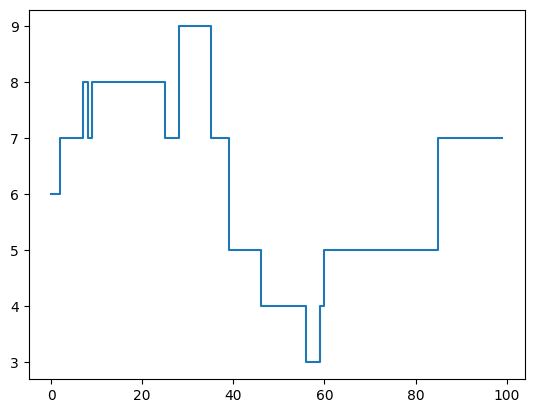
\includegraphics[width=\textwidth]{../pictures/2.f.1.png}
        \caption*{1 trajectory graph}
    \end{minipage}
    \hfill
    \begin{minipage}[b]{0.49\textwidth}
        \centering
        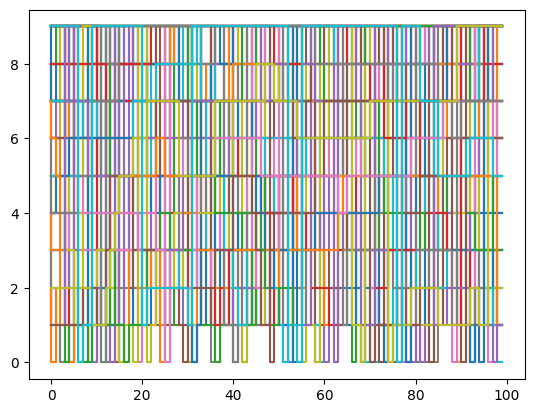
\includegraphics[width=\textwidth]{../pictures/2.f.2.png}
        \caption*{The graph mess for all the trajectories}
    \end{minipage}
\end{figure}

Finally, we estimate $\nu$ the same way we estimated $\mu$ previously by taking the frequencies of each state in all the trajectories

\[ \hat{\nu}_i = \frac{1}{m}\sum_{j = 0}^{m} \1(X^j = i) \]

\begin{minted}{python3}
    visit_frequencies = []
    for k in range(N):
        state_list = trajectories[k][:-1]
        values, indices, counts = np.unique(state_list[state_list.argsort()], return_counts=True, return_index=True)
        visit_frequency = np.zeros((10,))
        visit_frequency[values] = counts
        visit_frequencies.append(visit_frequency)
    average_visit_frequency = np.array(visit_frequencies).mean(axis = 0)
    average_visit_frequency = average_visit_frequency/average_visit_frequency.sum()

    bar_width = 0.35
    x = range(len(average_visit_frequency))

    fig, ax = plt.subplots()
    bar1 = ax.bar(x, average_visit_frequency, bar_width, label=r'$\hat{\nu}_i = \frac{1}{m}\sum_{j = 0}^{m} 1(X^j = i)$')
    bar2 = ax.bar([i + bar_width for i in x], transition_invariant, bar_width, label=r"$\nu_i$")

    ax.set_xticks([i + bar_width / 2 for i in x])
    ax.set_xticklabels([str(i) for i in range(len(average_visit_frequency))])
    ax.legend()
\end{minted}

\begin{figure}[H]
    \centering
    \begin{minipage}[b]{0.49\textwidth}
        \centering
        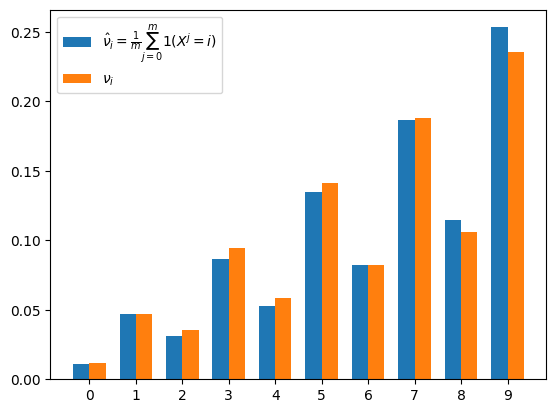
\includegraphics[width=\textwidth]{../pictures/2.f.3.png}
        \caption*{$N = 100,\; T = 100$}
    \end{minipage}
    \hfill
    \begin{minipage}[b]{0.49\textwidth}
        \centering
        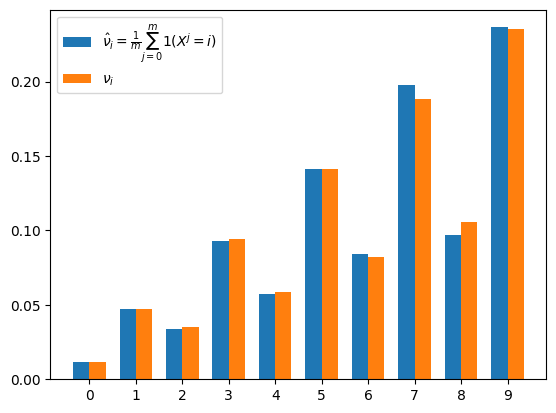
\includegraphics[width=\textwidth]{../pictures/2.f.4.png}
        \caption*{$N = 100,\; T = 1000$}
    \end{minipage}
    \caption*{The {\color{blue} blue bar (left)} is the result of the estimator {\color{blue}$\boldsymbol{\wh{\nu}_i}$} simulated $N=100$ times.\\ The {\color{red} orange bar (right)} is real value of the invariant measure {\color{red}$\boldsymbol{\nu_i}$}. }
\end{figure}
